\begin{recipe}
    [% 
        preparationtime = {\unit[30]{min}},
        portion = {\portion{3-4}},
        bakingtime = {\unit[30]{min}}
    ]
    {Carrot \textit{kopytka}}

    \introduction{%
        Potatoes are main ingredient of polish cusine.
        You can make all sorts of things out of them: kopytka, pyzy, kluski śląskie... This recipe, however, is even better - it incorporates carrots to add colour, flavour and nutrients.
        It's also a perfect dish to smuggle vegetable for a poor eater.
    }

    \ingredients{%
        \unit[500]{g} & Carrot purée \\
        \unit[200]{g} & Starch \\
        \unit[200]{g} & Corn flour \\
        2 tbs. & Yeast flakes \\
        & Nutmeg \\
        \textbf{Sauce} & \\
        5 & Garlic cloves \\
        2 tbs. & Tahini \\
        2 tbs. & Soy sauce \\
        \nicefrac{1}{2} & Lime \\
        2 tbs. & Sesame oil \\
        1 ts. & Coriander \\
        1 ts. & Cumin
    }

    \preparation{%
        \step  Boil 5l of water.

        \step Knead all ingredients for dough.
        Roll and cut into small rods (see picture).

        \step Cook \textit{kopytka} in hot water till tender
        (about 3 min from the moment when they started floating - as opposed to stay at the bottom of the pot).

        \step Heat frying pan with some oil.
        Add all ingredients of the sauce
        (do it in chunks if you're not going to fit all of the \textit{kopytka} at once).

        \step  Fry \textit{kopytka} and covered in sauce.
        Serve with greens.
    }

\end{recipe}

\begin{figure}[h]
    \centering
    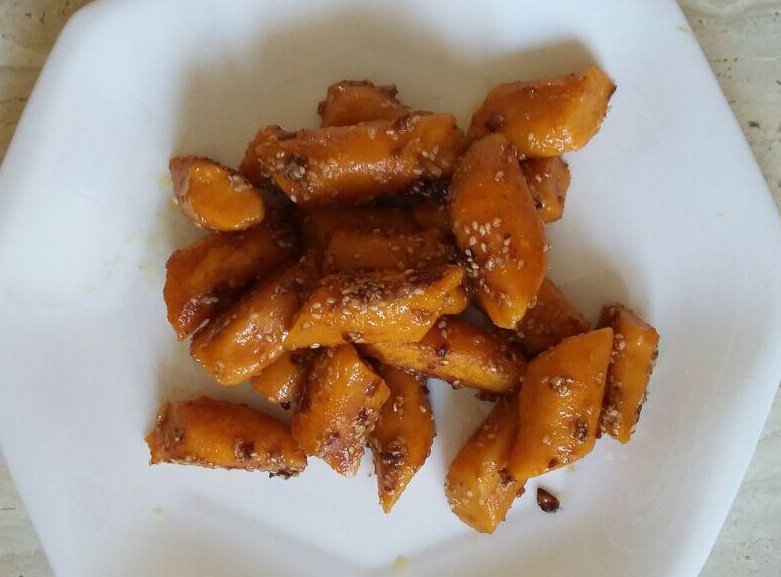
\includegraphics[width=8cm]{pic/carrot_kopytka}
\end{figure}

\begin{figure}[h]
    \centering
    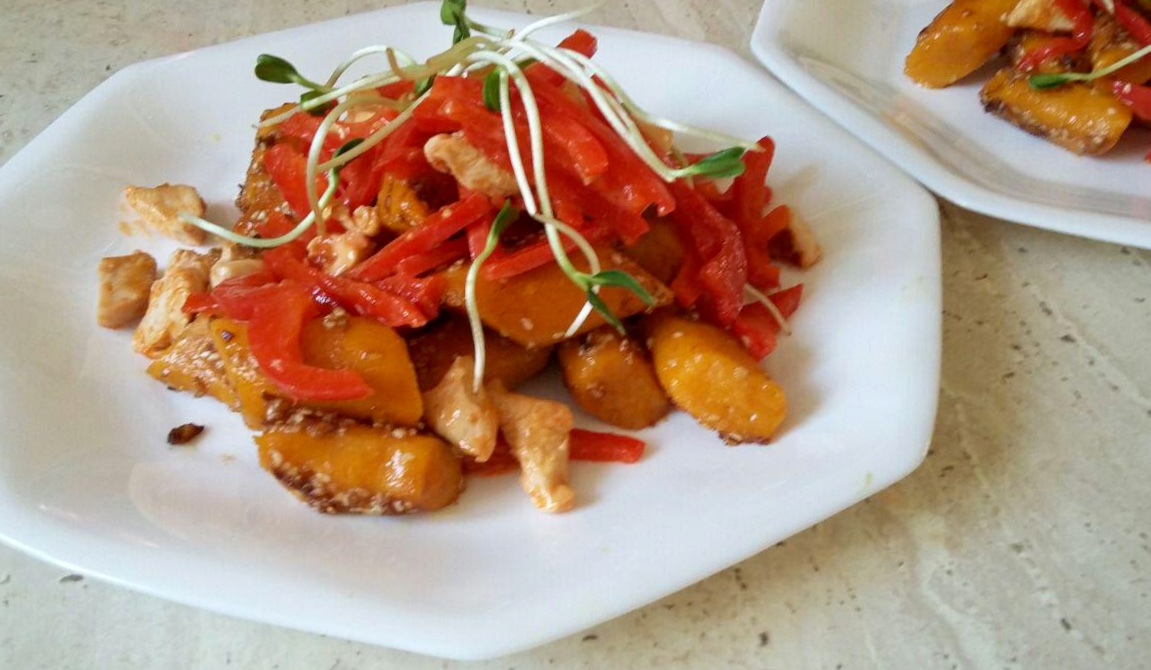
\includegraphics[width=8cm]{pic/carrot_kopytka_2}
\end{figure}

